\documentclass[times,specification,annotation]{itmo-student-thesis}

\usepackage{icomma}
\usepackage{tikz}
\usetikzlibrary{arrows}
\usepackage{filecontents}
\usepackage{rotating}

\addbibresource{bachelor-thesis-kate.bib}

\newcommand{\specialcell}[2][c]{%
  \begin{tabular}[#1]{@{}c@{}}#2\end{tabular}}
\newcommand{\specialcelll}[2][l]{%
  \begin{tabular}[#1]{@{}l@{}}#2\end{tabular}}

\begin{document}

\studygroup{P3420}
\title{Автоматическое выделение функциональных наборов генов в базе GEO с помощью дифференциальной экспрессии}
\author{Беляева Екатерина Сергеевна}{Беляева Е.С.}
\supervisor{Сергушичев Алексей Александрович}{Сергушичев А.А.}{к.т.н.}{доцент кафедры КТ}
\publishyear{2018}
\startdate{01}{декабря}{2017}
\finishdate{31}{мая}{2018}
\defencedate{18}{июня}{2018}

\secretary{Бутько Е.Ф.}

%% Задание
%%% Техническое задание и исходные данные к работе
\technicalspec{В рамках выпускной квалификационной работы основной задачей является построение функциональных наборов генов из базы GEO с помощью анализа дифференциальной экспрессии, а также обеспечение интерфейса доступа к ним}

%%% Содержание выпускной квалификационной работы (перечень подлежащих разработке вопросов)
\plannedcontents{\begin{enumerate}
    \item Обзор предметной области.
    \item Анализ существующих сервисов.
    \item Загрузка данных и их обработка.
    \item Построение модулей генов при помощи анализа дифференциальной экспрессии.
    \item Обеспечение интерфейса доступа к модулям генов.
    \item Анализ полученных результатов.
\end{enumerate}}

%%% Исходные материалы и пособия 
\plannedsources{\begin{enumerate}
    \item Bioconductor. Bioconductor is an open source, open development software project to provide tools for the analysis and comprehension of high-thoughput genomic data. [Электронный ресурс]. URL: https://www.bioconductor.org/;
    \item Docker. Docker is the software container platform. [Электронный ресурс]. URL: https://www.docker.com/;
    \item Терри А.Браун Геномы / Терри А.Браун. - М.-Ижевск: Институт компьютерных исследований, 2011. - 921 c.  
\end{enumerate}}

%%% Цель исследования
\researchaim{Получить новую базу функциональных наборов генов.}

%%% Задачи, решаемые в ВКР
\researchtargets{\begin{enumerate}  
    \item изучение существующих сервисов для работы с данными экспрессии генов;
    \item построение новых функциональных наборов генов из базы GEO при помощи анализа дифференциальной экспрессии;
    \item анализ полученных результатов;
    \item обеспечение интерфейса доступа к модулям генов.
\end{enumerate}}

%%% Использование современных пакетов компьютерных программ и технологий
\addstage{R (библиотеки GEOquery, limma, dplyr, stringr, data.table, magrittr, tibble)}{Глава 2, Глава 3}
\addstage{Python 2,3 (библиотеки pandas, subprocess, re, csv)}{Глава 2, Глава 3}
\addstage{Bash}{Глава 2, Глава 3}
\addstage{Kotlin}{Глава 3}
\addstage{Django}{Глава 3}
\addstage{Java Script}{Глава 3}
\addstage{React}{Глава 3}
\addstage{HTML}{Глава 3}
\addstage{CSS}{Глава 3}
\addstage{Docker}{Глава 3}

%%% Краткая характеристика полученных результатов 
\researchsummary{По итогу работы был реализован сервис с возможностью предоставления доступа к модулям генов конечному потребителю.}

%%% Гранты, полученные при выполнении работы 
\researchfunding{Грантов или других форм государственной поддержи и субсидирования в процессе работы не предусматривалось.}

%%% Наличие публикаций и выступлений на конференциях по теме выпускной работы
\researchpublications{Публикаций и выступлений на конференциях не было.}

\maketitle{Бакалавр}

%% Оглавление
\tableofcontents

%% Введение
\startprefacepage

Жизнь, какой мы ее видим, создается геномами мириад организмов, с которыми мы делим нашу планету. Каждый из этих организмов обладает геномом, содержащем биологическую информацию, необходимую для построения и поддержания организма живущего в настоящий момент времени представителя данного вида \cite{Introduction}. Изучением геномов занимается биоинформатика ~-- наука, стоящая на границе биологии и информатики, активно развивающаяся в течении последних десятилетий. Биоинформатика также связана с биохимией, биофизикой, экологией и многими другими областями. Открываются новые направления исследований, появляется всё больше данных, в том числе и открытых.

Геном ~-- хранилище биологической информации, но сам по себе он не способен выдать эту информацию клетке. Использование биологической информации, содержащейся в геноме, возможно лишь благодаря согласованным действиям ферментов и других белков, которые участвуют в сложной серии биохимических реакций, называемой экспрессией генома \cite{Introduction}.

Так, одним из направлений биоинформатики являются исследования, связанные с экспрессией генов, т.е. с процессом преобразования последовательности гена в функциональный продукт (обычно белок). Экспрессия гена может быть измерена количественно. Существует множество данных экспрессии генов. Самой известной и часто используемой базой данных экспрессии является база данных ​Gene Expression Omnibus (GEO). Она содержит данные о тысячах экспериментов, имеет сложную структуру. При этом каждый эксперимент также состоит из нескольких образцов, гены которых проаннотированы определенной пробой. GEO открытая, и именно она и будет использована в дальнейшей работе. 

Есть множество сервисов, работающих с данными экспрессии генов. В этой работе был рассмотрен и расширен сервис GeneQuery, который является поисковым порталом, использующим данные из базы GEO. Сервис плохо работал с маленькими по числу образцов датасетами, следовательно существовала проблема изменения принципа обработки данных. Так, целью данной бакалаврской работы являлось построение функциональных наборов генов из базы GEO с помощью дифференциальной экспрессии, т.е. при помощи наблюдения за изменением активности гена в зависимости от биологического состояния. Сервис GeneQuery был расширен для поддержки новых данных. Ожидается, что используя новую базу функциональных групп генов может быть выявлена потенциально значимая биологическая информация, а сам сервис может быть использован исследователями в области биоинформатики.        

%% Содержательная часть.
\chapter{ОБЗОР ПРЕДМЕТНОЙ ОБЛАСТИ}

\section{Основные понятия и определения}
\startrelatedwork
\textit{Биоинформатика} ~-- это междисциплинарная область, работающая с биологическими данными. Она сочетает в себе информатику, биологию, математику, статистику и ещё множество областей. Также широк и круг исследований биоинформатики, однако данная работа будет сосредоточена на таком направлении, как экспрессия генов.

\textit{Ген} ~-- единица наследственности живых организмов.

\textit{Экспрессия гена} ~-- процесс преобразования последовательности гена в функциональный продукт (обычно белок). Она может быть измерена количественно. 

\textit{Дифференциальная экспрессия гена} ~-- изменение уровня экспрессии гена в зависимости от биологического состояния.

\textit{Функциональная группа генов} ~-- отвечает за конкретное биологическое явление или несколько явлений. 

Для примера можно рассмотреть гликолиз ~-- процесс расщепления глюкозы в клетках, сопровождающийся синтезом АТФ. Для протекания этого процесса необходимы ферменты, т.е. ускорители химических реакций. В гликолизе участвуют ферменты гексокиназа, глюкозофосфатизомераза, енолаза и другие. Их структуры определяются генами HK1, PGI1, ENO1 \cite{Glycolysis} и т.д. Все эти гены являются функциональной группой генов для процесса гликолиз.

\textit{Фенотип} ~-- это совокупность всех характеристик конкретного организма в определенное время, стадии развития и окружающих факторов. Например, крыса в определенном возрасте с определенным заболеванием и цветом глаз является фенотипом. А крыса того же возраста и цвета глаз, но с другим заболеванием будет уже другим фенотипом. 

\section{База данных GEO}

Биоинформатика обладает большим объемом информации, который нужно где-то хранить. Для этой цели существуют множество баз данных. Накопление данных о генах, проявивших себя в биологических экспериментах, т.е. функциональных групп генов, является важной задачей потому, что эта информация может быть полезна в будущем. Самым известным открытым репозиторием для хранения данных экспрессии генов является \textit{Gene Expression Omnibus}. Или же сокращенно \textit{GEO}.

Проект GEO был инициирован в ответ на растущую потребность в общедоступном хранилище данных экспрессии генов \cite{GEO}. Эксперименты, хранящиеся в репозитории, имеют определенную структуру. Для каждого эксперимента представлены: 
\begin{itemize}
    \item GSM (Geo SaMple) ~-- \textit{образцы} или \textit{сэмплы} ~-- эти данные содержат информацию об организмах, участвовавших в эксперименте, об условиях эксперимента.
    \item GSE (Geo SEries) ~-- \textit{серия} ~-- объединяет в себе несколько образцов и хранит данные о числовых значениях экспрессии генов каждого образца. Как правило это ~20000 генов на каждый обзазец.
    \item GPL (Geo PLatform) ~-- \textit{платформа}, на которой вычислялась экспрессия. Важным компонентом, хранящимся здесь, является информация для каждого гена о соответствии его entrez к symbol.     
\end{itemize}

Количество данных GEO огромно и постоянно растет, в следствии чего база представляет исключительный интерес в биоинформатическом сообществе. Как было отмечено ранее, данная работа посвящена обработке данных именно из GEO.   

\section{Сервис GeneQuery}

Проект GeneQuery \cite{GeneQuery} - это поисковый портал, основанный на автоматическом выделении наборов генов с помощью кластеризации. Работает с данными экспрессии генов из базы данных GEO для организмов Homo Sapience, Mus Musculus и Rattus Norvegicus, т.е. с человеком, мышью и крысой. На вход сервису подается набор генов. Результатом запроса являются модули генов, перекрывающиеся с запросом пользователя, и проранжированные в порядке статистической значимости. Инструмент также показывает тепловые карты экспрессии генов для каждого найденного модуля. 
Взаимодействие элементов сервиса представлено на рисунке~\ref{GeneQuery_service}. 

\begin{figure}[!h]
    \caption{Схема сервиса.}\label{GeneQuery_service}
    \centering
    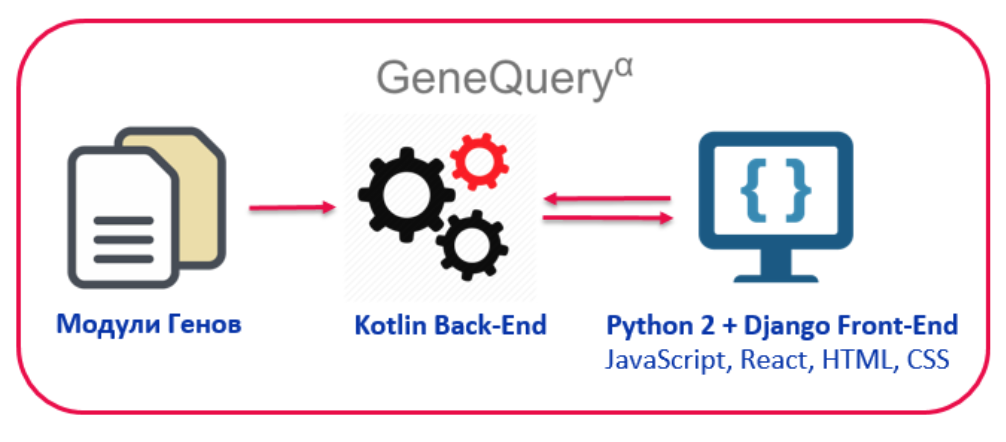
\includegraphics[width=0.9\textwidth]{GeneQuery_scheme}
\end{figure} 

GeneQuery имеит такие достоинства, как высокая скорость обновления данных (новые данные из GEO можно портировать в GeneQuery), быстрая скорость выдачи результата для пользователя, простота использования. Сервис достаточно хорошо работает для средних по размеру датасетов (по числу образцов), но не подходит для маленьких. Для последних можно использовать анализ дифференциальной экспрессии, что и сделано в альтернативной версии GeneQuery - в GeneQueryDE. 

\section{Сервис GEOracle}

GEOracle \cite{GEOracle} ~-- инструмент для поиска данных по экспрессии генов по базе GEO, открытый для использования летом 2017 года. Использует технологии машинного обучения для автоматического выделения нужных экспериментов, их объединения в группы и подсчета дифференциальной экспрессии \cite{GEOracleArticle}. Сервис получает на вход набор экспериментов, а в результате их обработки, выдает значения экспрессии генов в зависимости от указанного фактора и, также, показывает тепловые карты зависимости экспериментов от генов.

\section{Сервис ARCHS4}

ARCHS4 \cite{ARCHS4} ~-- сервис с обширным функционалом. Работает с данными видов Homo Sapience и Mus Musculus. Имеет функции поиска, позволяющие просматривать данные с помощью аннотаций метаданных, сходства структур и функциональной представленности \cite{ARCHS4help}. Также сервис позволяет визуализировать данные в 3D представлении. На вход может получать ген либо набор генов в верхней/нижней регуляции (как дополнительные параметры можно указать ткани, органы). Результатом запроса станут данные о гене, средняя экспрессия, отображение данных на 3D модели. Сервис также позволяет загружать полученные результаты. 

\section{Сервис GEO Profiles}

GEO Profiles \cite{GEOprofiles} ~-- это инструмент поиска по базе GEO. Обладает широкими возможностями, подразумевая то, что, как и в обычном поисковике, можно вводить любой текст в надежде получить результат. В данном поисковике запросом может быть свободный текст, но также существуют некие шаблоны ввода. Например, можно искать конкретный ген, эксперимент или организм. А можно какую-то комбинацию выше написанного. В зависимости от запроса пользователь может получить информацию об эксперименте со ссылкой на него, информацию о платформах экспериментов, информацию о генах и многое другое. Также стоит отметить, что GEO Profiles снабжен достаточно полной документацией, что позволяет быстро разобраться в особенностях работы с ним.

\section{Язык программирования R}

R ~-- это бесплатная программная среда для статистических вычислений и графики \cite{R}. Он работает под платформами UNIX, Windows и MacOS. Язык поддерживается большим сообществом разработчиков и активно используется для статистики и анализа данных. Также широко он применяется в биоинформатике. На R написаны десятки библиотек для биоинформатического анализа данных, для работы с базами данных в этой области, а также для представления результата. Проект, объединяющий в себе полезные пакеты для работы с базой GEO называется Bioconductor. Он и был использован в данной работе.

\section{Тест Фишера}

Тест Фишера ~-- это тест статистической значимости, используемый для анализа таблиц сопряженности, т.е. таблиц в матричной форме, отображающих распределения переменных \cite{Fisher}. Тест используется для изучения случайности связи между двумя видами классификации данных и применяется для категориальных данных, представляющих из себя результат классификации.

\section{P-значение}

P-значение (P-value) ~-- величина, которая используется для тестирования статистических гипотез и является одним из возможных методов оценки вероятности ошибки при отклонении нулевой гипотезы.

\section{Поправка Бонферрони}

Одна из мер, позволяющих получить групповую вероятность ошибки первого рода. Данный метод основан на формуле: 

\begin{equation}
\label{bonferroni}
    p_{i} < \frac{\alpha }{m}
\end{equation}

, где \begin{math}p_i\end{math} ~-- вероятность \textit{i}-го события, 

\textit{m} ~-- количество событий,

\textit{α} ~-- порог значимости ~-- некоторое число (в данной работе = 0.01).

Использование формулы\ref{bonferroni} позволяет отклонить гипотезы, неудовлетворяющие ей, т.е. уменьшить колличество ложноположительных результатов \cite{Bonferroni}.

\section{Контейнеризация}

Контейнеризация ~-- упаковывание в контейнер, т.е. в тип, позволяющий инкапсулировать в себе объекты других типов \cite{Containerization} и запущенный в изолированном окружении. Одной из самых популярных технологий контейнеризации является Docker \cite{Docker}, предоставляющий удобный интерфейс для управления контейнером. 

Docker ~-- это открытый проект для разработки и эксплуатации приложений, разработанная для быстрого выкладывания приложений. При помощи легковесной платформы контейнерной виртуализации, используя процессы и утилиты, помогающие управлять и выкладывать приложения \cite{DockerUnderstanding}, docker отделяет приложение от инфраструктуры и позволяет обращаться с инфраструктурой как с управляемым приложением. Технология docker позволяет запускать приложение, безопасно изолированное в контейнере. Более того, безопасная изоляция позволяет запускать на одном хосте много контейнеров одновременно. 

Docker включает в себя три основных компонента: образы(images), реестр(registries) и контейнеры.

Docker-образ ~-- это шаблон read-only, являющийся компонентой сборки. Например, образ может содержать операционную систему Ubuntu c java-машиной и приложением на ней. Образы нужны для создания контейнеров. Docker позволяет создавать новые образы, обновлять те, что есть. Также образы можно скачивать, подразумевая то, что они были созданны другими людьми. Для создания образа пишется Dockerfile.

Docker-реестр ~-- это место хранения образов, являющееся компонентой распростронения. Есть приватные и публичные реестры, из которых можно скачать или в которые загружать образы. Публичный Docker-реестр ~-- это Docker Hub \cite{DockerHub}, где хранится большая коллекция образов.

Контейнеры похожи на папки с данными ~-- это компонента работы. Так, в контейнерах находится все, что нужно для работы приложения ~-- операционная система, требуемые программные зависимости, само приложение. Каждый контейнер создается из образа. Контейнеры можно создавать, запускать, останавливать, переносить или удалять. Каждый контейнер изолирован и является безопасной платформой для приложения.

\section{Цель и актуальность работы}

Учитывая то, что сервис GeneQuery плохо работает с маленькими по числу образцов экспериментами, требовалось изменить механизм работы сервиса. Так целью данной работы было построение наборов генов по экспериментам из базы GEO c помощью анализа дифференциальной экспрессии и обеспечение интерфейса доступа к ним. 

Портал GeneQuery расширен для поддержки новых данных до версии GeneQueryDE. Сервис может быть использован исследователями в области биоинформатики. Ожидается, что используя новую базу функциональных групп генов может быть выявлена потенциально значимая биологическая информация. 

\section{Задачи}

Основываясь на цели, обозначенной в предыдущем пункте, были выделены следующие задачи, решенные в ходе работы:
\begin{itemize}
    \item Выгружены данные экспериментов и аннотаций из GEO.
    \item Данные обработаны.
    \item Построены наборы генов с помощью анализа дифференциальной экспрессии.
    \item Осуществленна поддержка новых данных сервисом GeneQuery.
    \item Сервис запущен для массового использования.
\end{itemize}

\chapterconclusion

В данной главе был произведен обзор предметной области. А именно, рассмотрены основные биологические понятия, являющиеся базовыми для понимания дальнейших действий. Рассмотрены применненные технологии и сервисы, на которых строится данная работа. Также обозначены цели работы и ее значимость, показаны задачи, решаемые для достижения цели. 
\finishrelatedwork

\chapter{ПОСТРОЕНИЕ МОДУЛЕЙ ГЕНОВ}

\section{Загрузка данных}

База данных GEO имеет сложную структуру. Например, датасет GSE61055 находится по адресу \textit{https://ftp.ncbi.nlm.nih.gov/geo/series/GSE61nnn/GSE61055/matrix/} \textit{GSE61055\_series\_matrix.txt.gz}, а аннотация к нему лежит на \textit{https://ftp.ncbi.nlm.nih.gov/geo/platforms/GPL6nnn/GPL6887/annot/} \textit{GPL6887.annot.gz}. При скачивании данных, структура GEO была сохранена. Для загрузки использовались языки Python 3 и Bash. 

\begin{lstlisting}[float=!h, caption={Загрузка данных из GEO.}, captionpos=b, label={downloadGEO}, basicstyle=\footnotesize, language=Python]
import subprocess
import csv

def download_data(file_name, kind_data): 
    with open(file_name,'r') as tsvin:
        tsvin = csv.reader(tsvin, delimiter='\t')
        indexes = []
        
        for (i, row) in enumerate(tsvin):
            if i == 0:
                if kind_data == 'series':
                    indexes = [row.index(j) for j in ['Series', 'Series_url']]
                else:
                    indexes = [row.index(j) for j in ['Platforms', 'Platforms_url']]
            else:    
                try:
                    dif_string = 'https://ftp.ncbi.nlm.nih.gov/'
                    path = row[indexes[1]].replace(dif_string, '')
                    path = path[:(path.rindex('/')+1)]
                    directory = "../" + path

                    subprocess.call(["mkdir", "-p", directory])
                    subprocess.call(["wget", "-c", "-P", directory, row[indexes[1]]])

                except:
                    pass

\end{lstlisting}


Основная функция загрузки приведена на листинге~\ref{downloadGEO}. Всего было загружено 74177 датасетов типа GSE (с экспрессией генов) и 790 GPL (аннотаций) для видов Homo Sapience, Mus Musculus и Rattus Norvegicus. 

Примеры данных типа GSE и GPL приведены на рисунках~\ref{GSE61055} и ~\ref{GPL6887} соответственно. 

\begin{figure}[!h]
    \caption{Таблица с экспрессией генов для GSE61055.}\label{GSE61055}
    \centering
    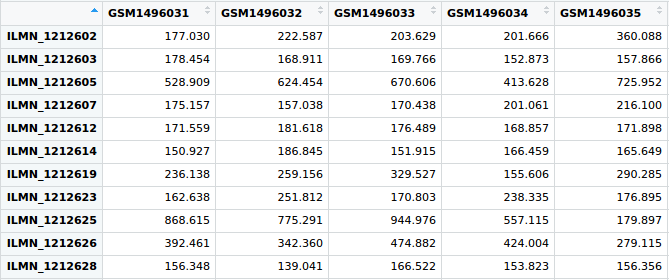
\includegraphics[width=0.9\textwidth]{GSE61055.png}
\end{figure}  

\begin{figure}[!h]
    \caption{Аннотация GPL6887.}\label{GPL6887}
    \centering
    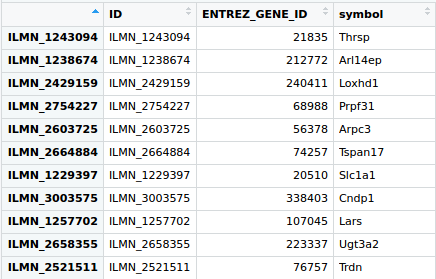
\includegraphics[width=0.7\textwidth]{GPL6887.png}
\end{figure} 

Далее GSE были сопоставлены с аннотациями и выяснилось, что 29098 датасетов пригодно для построения таблиц ​дифференциальной экспрессии.


\section{Автоматическая обработка}

После получения таблицы с матчингом GSE с GPL, для каждого эксперимента надо было построить модули генов с применением анализа дифференциальной экспрессии. Для этого, для каждого датасета были выполнены действия:
\begin{itemize}
    \item Выявлены уникальные условия каждого эксперимента.
    \item Сопоставлены пробы и гены.
    \item Нормализованны данные.
    \item Построены пары условий.
    \item Построены таблицы дифференциальной экспрессии.
\end{itemize}

Для всего вышеперичисленного использовался язык R с применением инструмента Bioconductor. Bioconductor ~-- это проект на R, содержащий множество библиотек для анализа геномных данных \cite{Bioconductor}. В том числе имеет библиотеку для взаимодействия с базой данных GEO. Так, работая на R, были использованы пакеты GEOquery и limma. 

\subsection{Выявление уникальных условий каждого эксперимента}

GSE датасет содержит таблицу с указанием информации по каждому образцу, участвовавшему в эксперименте. В том числе, содержатся условия эксперимента для каждого образца. Эти данные записаны в столбцах <<charactericstics>>, которых может быть от 1 до n. Требовалось автоматически выделять биологические состояния.  

Поиск нужных для парсинга столбцов на листинге~\ref{searchCharacteristicsColumns}. 

\begin{lstlisting}[float=!h, caption={Поиск столбцов <<charactericstics>>.}, captionpos=b, label={searchCharacteristicsColumns}, basicstyle=\footnotesize, language=R]

getCharacteristicsColumns <- function(gse) {
  col <- colnames(pData(gse))
  characteristics <- c()
  for (ch in col) {
    if (grepl("characteristics", ch)) characteristics <- c(characteristics, ch)
  }
  return(characteristics)
}

\end{lstlisting}

Рассматриваемый столбец не должен был быть пустой или содержать NA, т.ч. сначала были отобраны колонки, удовлетворяющие этим условиям. Далее нужно было оставить только значимые состояния. В колонках <<charactericstics>> мог быть написан любой текст, содержащий любые символы и цифры. Прежде всего надо было убедиться, что в столбце написано не простое перечисление номеров образцов. Такие столбцы исключались из рассмотрения. На листинге~\ref{checkImportanceCharacterictics} приведена проверка на значимость цифр. Если массив цифр, отсортированный по возрастанию, содержал целые, не дублирующиеся цифры и имел на концах значения единицы и количества образцов, то такие цифры признавались простым перечислением номеров образцов, и содержащий их столбец дальше в построении условий не участвовал.    

\begin{lstlisting}[float=!h, caption={Проверка значимости столбца <<charactericstics>>.}, captionpos=b, label={checkImportanceCharacterictics}, basicstyle=\footnotesize, language=R]

isUsefulNumbers <- function(numbers) {
  maxNumber <- length(numbers)
  numbers <- sort(numbers, decreasing = F)
  
  isInteger <- T
  tryCatch({
    stopifnot(all(numbers == floor(numbers)))
  }, error = function(e) {
    isInteger <- F
  })
  
  isUseful <- T
  if (isInteger && numbers[1] == 1 && numbers[maxNumber] == maxNumber 
      && length(unique(numbers)) == maxNumber) 
    isUseful <- F
  
  return(isUseful)
}

getConditionsFromUniqValues <- function(charColumns, conditionsList, 
                                              explanatoryTable, usedMarkers) {
  values <- sub("^.*: ", "", charColumns[[1]])
  numerics <- is.na(suppressWarnings(as.numeric(values)))
  
  if ((length(numerics[numerics==FALSE]) == 0) || 
      (length(numerics[numerics==FALSE]) != 0 && isUsefulNumbers(as.numeric(values)))) {
    
    tmpCondition <- c()
    beforeColon <- gsub(" ", ".", sub(":.*", "", charColumns[[1]]))
    values <- paste(beforeColon, ".", values, sep="")
    
    ...

\end{lstlisting} 

Следующая проблема, которую надо было решить, заключалась в работе с длинными последовательностями текста в <<charactericstics>>, т.е. в обработке сложных условий. Условие признавалось сложным, если в нем было больше некоторого количества определенных знаков (листинг~\ref{isTooComplicatedCondition}). Такие условия обрабатывались определенным способом. Это было сделано не только из-за того, что явное использование некоторых символов приводило к ошибкам заполнения неких структур для построения дифференциальной экспрессии, но также и из-за эстетических соображений и восприятия (т.к. в конечном счете из каждого <<простого>> условия удалялись все <<сомнительные>> символы, а пробелы заменялись на точки).     

\begin{lstlisting}[float=!h, caption={Проверка сложности условия.}, captionpos=b, label={isTooComplicatedCondition}, basicstyle=\footnotesize, language=R]

isTooComplicatedCondition <- function(condition) {
  if (length(unlist(gregexpr(pattern = "\\+", condition))) > 1
      || length(unlist(gregexpr(pattern = "-", condition))) > 1
      || length(unlist(gregexpr(pattern = " ", condition))) > 1)
    return(TRUE)
  return(FALSE)
}

\end{lstlisting} 

Так как по результату работы программы создавались файлы модулей генов с подписями условий, по которым была вычисленна дифференциальная экспрессия, то нужно было быть аккуратным с символами, которые можно записывать в название, ведь не все символы допускаются для названия файла. По этой причине и также по причине, описанной выше, некоторые символы удалялись из условия, а пробелы заменялись на точки (листинг~\ref{cleaning}).  

\begin{lstlisting}[float=!h, caption={Удаление некоторых символов и замена пробелов на точки.}, captionpos=b, label={cleaning}, basicstyle=\footnotesize, language=R]

v <- gsub("[-\\+\\/;:\\.\\?!,\\\\]", ' ', v) %>% 
             gsub("\\s+", ' ', .) %>% 
             gsub("(^\\s+)|(\\s+$)", '', .) %>% 
             gsub(" ", ".", .)

\end{lstlisting} 

Немного не так обстояла ситуация со <<сложными>> условиями. Эти условия не подвергались чистке символов, т.к. каждому такому условию присваивалась буква (или комбинация букв), под которой условие сохранялось в специальном файле со списком всех подобных условий (explanatoryTable). Файлы модулей генов в этом случае содержали эти буквы, а не исходный текст биологического состояния. Генерация маркеров для возможных <<сложных>> условий представлена на листинге~\ref{createMarkersForComplicatedConditions}.  

\begin{lstlisting}[float=!h, caption={Генерация маркеров для замены <<сложных>> условий.}, captionpos=b, label={createMarkersForComplicatedConditions}, basicstyle=\footnotesize, language=R]

createMarkersForComplicatedConditions <- function() {
  usedMarkers <- list()
  for (i in 1:26) usedMarkers[intToUtf8(64+i)] <- 0
  
  extraMarkers <- permutations(
    n=12, r=2, v=names(usedMarkers)[1:12], set=T, repeats.allowed=T)
  
  for (i in 1:(length(extraMarkers))/2) {
    cond <- paste(extraMarkers[[i,1]], extraMarkers[[i,2]], sep="")
    usedMarkers[cond] <- 0
  }
  return(usedMarkers)
}

\end{lstlisting} 

\begin{lstlisting}[float=!h, caption={Добавление условий в explanatoryTable.}, captionpos=b, label={addConditionToExplanatoryTable}, basicstyle=\footnotesize, language=R]

handleComplicatedCondition <- function(cond, explanatoryTable, usedMarkers) {

  newConditionName <- isContainedInExplanatoryTable(explanatoryTable, cond)
  if (newConditionName == "") {
    markerUse <- getFreeMarker(usedMarkers)
    newConditionName <- markerUse$marker
    usedMarkers <- markerUse$usedMarkers
    
    explanatoryTable <- rbindlist(list(explanatoryTable, data.table(
      "characteristics"=cond, "marking"=newConditionName)))
  }
  return(list("condition"=newConditionName, 
              "explanatoryTable"=explanatoryTable,
              "usedMarkers"= usedMarkers))
}

...

if (isTooComplicatedCondition(v)) {
    resultCondition <- handleComplicatedCondition(oldV, 
                              explanatoryTable, usedMarkers)

\end{lstlisting}

Обработанные условия из каждого столбца <<charactericstics>> для каждого образца затем соединялись вместе через символ <<\_>>. Например, как здесь: \textit{ATF3.deficiency\_IFNbeta}.

Как можно видеть на листинге~\ref{fillGseConditionColumn}, возможна ситуация, когда уникальные биологические состояния выделить не удавалось. Это могло быть связано с пропусками данных в столбцах <<charactericstics>> или же с тем, что условия не несли в себе универсального значения. Например, в датасете, состоящем из восьми образцов, в одной из колонок <<charactericstics>> могли быть написаны цифры от 1 до 8, соответствующие просто номерам образцов. Как было написано ранее, такие случаи игнорировались и не участвовали в дальнейшем анализе.   

\begin{lstlisting}[float=!h, caption={Выделение условий.}, captionpos=b, label={fillGseConditionColumn}, basicstyle=\footnotesize, language=R]

characteristics <- getCharacteristicsColumns(gse)
conditionLists <- list()

...

if (length(characteristics) > 0) {
    message("There are characteristics columns in the samples table.")
    conStructure <- getConditionsFromCharacteristics(gse, characteristics)
    conditionLists <- conStructure$conditionsList
    explanatoryTable <- conStructure$explanatoryTable 
  }
  
  if (length(conditionLists) > 0 && length(unique(unlist(conditionLists))) > 1) {
    pData(gse)$condition <- fillGseConditionColumn(conditionLists) 
    ...

  } else 
    message("Characteristics columns in the samples table don't exist or were unhelpful.")

\end{lstlisting}

Все выявленные состояния были сохранены в столбце <<condition>>, из которого затем были построены пары состояний и, основываясь на этом, модули с дифференциальной экспрессией генов.

\subsection{Сопоставление проб и генов}

Как можно видеть на рисунке~\ref{GPL6887} аннотация к чипу содержит id проб, генов и названия генов. Однако данные в таблице могут дублироваться. Чтобы избежать неточностей, было решено удалить дубликаты данных и рассматривать только уникальные значения (листинг~\ref{createGenesSymbolsTable}).

\begin{lstlisting}[float=!h, caption={Выделение условий.}, captionpos=b, label={createGenesSymbolsTable}, basicstyle=\footnotesize, language=R]

createGenesSymbolsTable <- function(gpl) {
  gpl <- read.table(gpl, header = T, sep = "\t",
                    colClasses = c("character", "character", "integer"))
  gpl <- gpl[!duplicated(gpl$id),]
  gpl <- gpl[!duplicated(gpl$gene_id),]
  
  gpl <- gpl %>% 
    set_rownames(.$id) %>% 
    select(ID = id, ENTREZ_GENE_ID = gene_id, symbol = gene_symbol)

  return(gpl)
}

\end{lstlisting}

Используя данные типа GSE (как на рисунке~\ref{GSE61055}) и GPL (рисунок~\ref{GPL6887}), на листинге~\ref{get7000} выделяются 7000 генов с наибольшей экспрессией, а также к таблице добавляются данные о entrez генов и их symbol, основываясь на сопоставлении проб. На основе этого набора генов в 7000 в дальнейшем строются модули с дифференциальной экспрессией. 

\begin{lstlisting}[float=!h, caption={Выделение 7000 генов с максимальной экспрессией.}, captionpos=b, label={get7000}, basicstyle=\footnotesize, language=R]

collapseData <- function(gse, gpl, FUN=median) {
  ranks <- apply(exprs(gse), 1, FUN)
  ranks <- data.frame(r = ranks, i = seq_along(ranks))
  table <- inner_join(rownames_to_column(gpl), rownames_to_column(ranks), 
           by="rowname") %>% 
           mutate(j = seq_along(symbol))
  t <- table[order(table$r, decreasing=T), ][1:7000,]
  keep <- t$i
  res <- gse[keep, ]
  rownames(res) <- table$ENTREZ_GENE_ID[t$j]
  fData(res)$symbol <- t$symbol
  return(res)
}

...

es <- collapseData(gse, gpl)

\end{lstlisting}    

\subsection{Нормализация данных}

В процессе обработки данных были совершены следующие действия:
\begin{itemize}
    \item Убраны дублирующиеся данные​.
    \item Убраны данные с пропусками​.
    \item Отобраны 7000 генов с самой высокой экспрессией​ (листинг~\ref{get7000}).
    \item Логарифмизация данных при большом размахе значений экспрессии (листинг~\ref{normalizeData}).
\end{itemize}

\begin{lstlisting}[float=!h, caption={Логарифмизация данных.}, captionpos=b, label={normalizeData}, basicstyle=\footnotesize, language=R]

if (max(exprs(es)) - min(exprs(es)) > 100)
        exprs(es) <- normalizeBetweenArrays(log2(exprs(es)+1), method="quantile")

\end{lstlisting} 

Как правило, после удаления дублирующихся данных и данных с пропусками в рассмотрении оставался набор, состоящий примерно из 20000 генов.

\subsection{Построение пар условий}

Так как дифференциальная экспрессия ~-- это изменение активности гена в зависимости от конкретного биологического состояния, то на данном этапе требовалось составить пары условий с различием в одно состояние. Для этого обрабатывался столбец \textit{pData(gse)\$condition}, получение которого показано на листинге~\ref{fillGseConditionColumn}.

Так, например парой условий является пара \textit{ATF3.deficiency\_IFNbeta} против \textit{ATF3.deficiency\_untreated}, где различно биологическое состояние \textit{IFNbeta} и \textit{untreated}.

\subsection{Построение таблиц дифференциальной экспрессии}

Для каждой пары условий, полученной по результатам предыдущего пункта, требовалось построить таблицу с дифференциальной экспрессией. Построение показано на листинге~\ref{fitLinearModel}. При помощи функции \textit{lmFit} заполняется линейная модель на основе данных об экспрессии генов и дизайн-матрицы. Дизайн-матрица ~-- это таблица с образцами в строчках и условиями в столбцах. В ячейке стоит 1, если условие соответствует данному образцу и 0, если в данном образце его нет. 

Далее вызывалась функция \textit{fitLinearModel}, на вход которой подавались линейная модель, пары условий, дизайн-матрица и количество обрабатываемых генов. Для каждой пары условий строилась контрастная матрица, на основе нее вычислялись расчетные коэффициенты линейной модели. Далее для модели расчитывалась эмпирическая Баесова статистика, включающая t-статистику, p-value и т.д. По просшествии данных преобразований, модель представлялась в виде таблицы с данными дифференциальной экспрессией генов.

\begin{lstlisting}[float=!h, caption={Построение модулей генов при помощи дифференциальной экспрессии.}, captionpos=b, label={fitLinearModel}, basicstyle=\footnotesize, language=R]

es.design <- model.matrix(~0+condition, data=pData(es))
fit <- lmFit(es, es.design)
deSize <- dim(exprs(es))[1]

...

fitLinearModel <- function(fit, conditions, design, deSize) {
  deList <- list()
  for (i in 1:length(conditions)) {
    
    contrasts <- makeContrasts2(
               c("condition", conditions[[i]]$firstCon, conditions[[i]]$secondCon), 
               levels=design)
    
    fit2 <- contrasts.fit(fit, contrasts)
    
    df.residual <- unique(fit2$df.residual)
    if ((length(df.residual) == 1 && df.residual[1] != 0) ||
        (length(df.residual) != 1)) {
      
      fit2 <- eBayes(fit2)
      
      deList[[i]] <- data.table(
        topTable(fit2, adjust.method="BH", number=deSize, sort.by = "B"), 
        keep.rownames = T)
    }
  }
  return(deList)
}

\end{lstlisting} 

Пример таблицы приведен на рисунке~\ref{difExprs}. Модуль содержит 7000 генов и включает в себя информацию о entrez гена, его названии, средней экспрессии и различные статистические метрики. 

Модули получилось построить для 15956 экспериментов.

\begin{figure}[!h]
    \caption{Таблица дифференциальной экспрессии генов.}\label{difExprs}
    \centering
    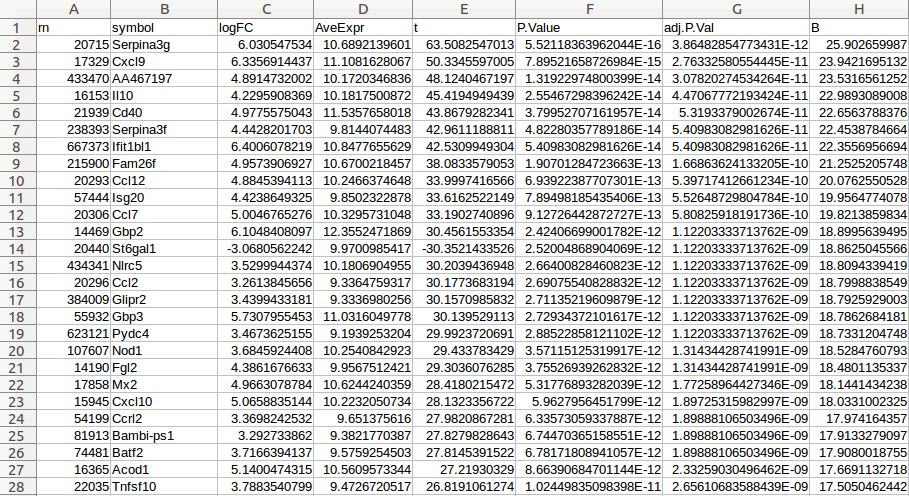
\includegraphics[width=1\textwidth]{difExprs.jpg}
\end{figure}

\section{Верхняя и нижняя регуляции генов}

Верхняя и нижняя регуляция генов ~-- это сравнение их активностей относительно друг друга. На предыдущем этапе были постоены таблицы генов при противопоставлении двух разных биологических состояний. Так, на данном этапе для каждого из модулей дифференциальной экспрессии генов требовалось построить дескриптивную выборку. По максимальному значению t-статистики отбиралось 200 генов, что соответствует верхней регуляции и по минимальному значению t-статистики отбиралось 200 генов, соответствующих нижней регуляции (листинг~\ref{200genes}). Полученные модули сохранялись. 

\begin{lstlisting}[float=!h, caption={Получение модулей по 200 генов.}, captionpos=b, label={200genes}, basicstyle=\footnotesize, language=R]

gse <- read.table(nameTables, header=T, sep="\t", 
                      fill = TRUE, quote = "", colClasses=colTypes)

up <- gse[order(gse$t, decreasing=TRUE),][1:200,]
down <- gse[order(gse$t),][1:200,]

\end{lstlisting} 

На основе модулей строились \textit{.gmt} файлы (рисунок~\ref{gmt}) для каждого вида (человек, мышь, крыса). Файлы содержали гены из экспериментов. А именно, для каждого эксперимента было представленно название, универсум (7000 генов), номера модулей и соответствующие выборки по 200 генов. Для каждого \textit{.gmt} файла был построен файл с аннотацией (рисунок~\ref{annot}), содержащий название эксперимента с номером модуля и название модуля.

\begin{figure}[!h]
    \caption{Пример \textit{.gmt} файла.}\label{gmt}
    \centering
    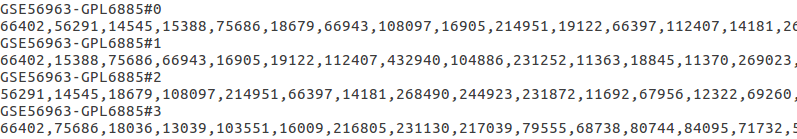
\includegraphics[width=1\textwidth]{gmt.png}
\end{figure}

\begin{figure}[!h]
    \caption{Пример аннотации к \textit{.gmt} файлу.}\label{annot}
    \centering
    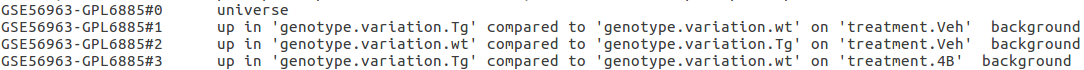
\includegraphics[width=1\textwidth]{gmt_annot.png}
\end{figure}

По итогам выборок по 200 генов, всего было получено 844324 новых модуля, которые затем были встроены в обработку сервиса GeneQueryDE.

\chapterconclusion

В данной главе был описан основной этап работы, который заключался в загрузке данных из базы GEO и построении модулей генов. Приведены цифры обработки данных и итоговые результаты.  


\chapter{WEB-СЕРВИС ДЛЯ ПОИСКА ФЕНОТИПОВ В МОДУЛЯХ ПО ДИФФЕРЕНЦИАЛЬНОЙ ЭКСПРЕССИИ}

После получения модулей генов, \textit{.gmt} файлов и файлов с аннотациями требовалось расширить сервис GeneQuery для возможности работы с новыми данными. Так была создана версия проекта GeneQueryDE. 

\section{Схема сервиса}

Взаимодействие элементов системы представлено на рисунке~\ref{service}. 

\begin{figure}[!h]
    \caption{Схема сервиса GeneQueryDE.}\label{service}
    \centering
    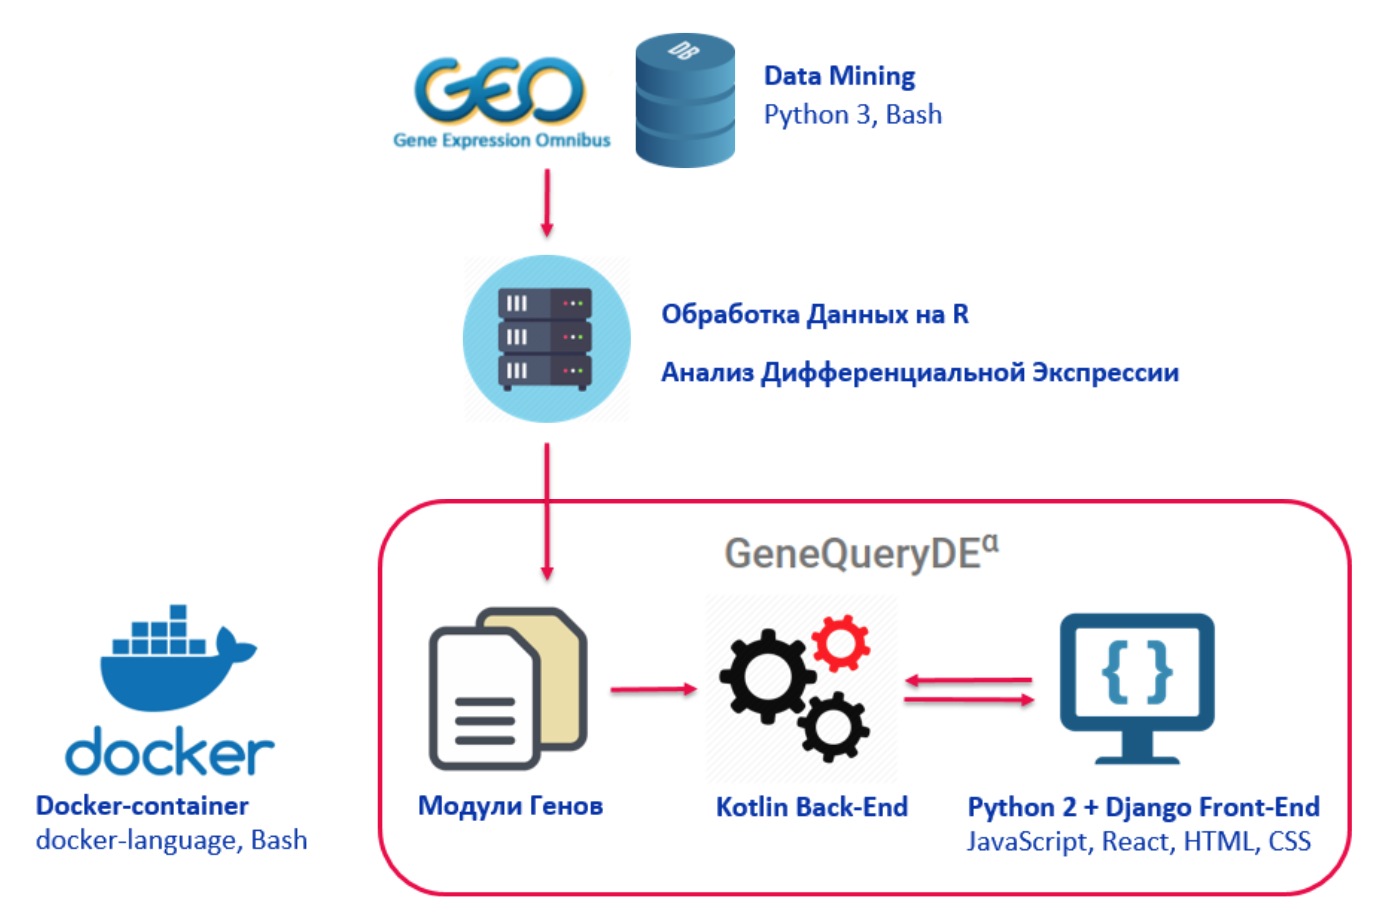
\includegraphics[width=0.9\textwidth]{GeneQueryDE_scheme}
\end{figure}

Подводя итог всему выше сделанному, с начала данные были загружены из базы GEO на сервер. Для этого использовались языки Python 3 и Bash. Далее на сервере происходила их обработка, и при помощи анализа дифференциальной экспрессии строились модули генов. Для этого использовался язык R.

После того, как модули генов были построены, сервис GeneQuery был расширен для поддержки новых данных до версии GeneQueryDE. Сам сервис состоит из двух репозиториев - front-end части на Python 2 + Django и back-end части на Kotlin. После, GeneQueryDE с новыми данными был упакован в docker-контейнер и запущен. Сейчас сервис доступен по адресу \textit{http://genome.ifmo.ru/genequery-de}.

\section{Back-end часть}

На рисунке~\ref{genequery-kotlin} показаны основные элементы структуры back-end репозитория GeneQueryDE. 

\begin{figure}[!h]
    \caption{Back-end часть GeneQueryDE.}\label{genequery-kotlin}
    \centering
    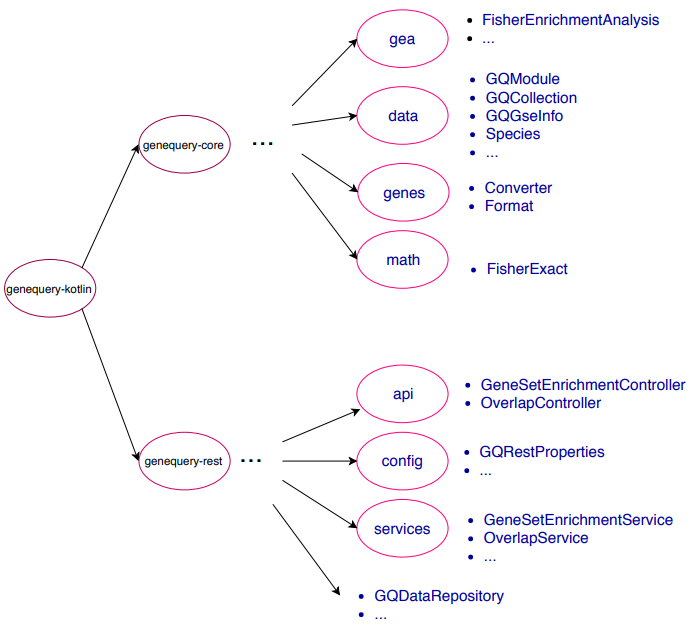
\includegraphics[width=1\textwidth]{genequery-kotlin.png}
\end{figure}

Как можно видеть, внутри себя проект разделяется на две логические составляющие ~-- \textit{genequert-rest} и \textit{genequery-core}, связанные соответственно с взаимодействием с front-end частью и обеспечивающие базовый функционал. Каждая составляющая имеет сложную иерархию пакетов. Основные из них показаны на рисунке. Также на схему вынесены главные файлы, содержащиеся в данных пакетах.  

\subsection{Пакет \textit{data}}
Пакет содержит такие файлы как \textit{GQModule}, \textit{GQCollection}, \textit{GQGseInfo}, \textit{Species} и т.д., отвечающие за хранение и доступ к разным структурам вроде модулей генов, экспериментов, видов организмов. 

Класс \textit{GQModule} представляет объект модуля. Модули инициализируются при старте приложения и чтении \textit{.gmt} файлов с аннотациями. Класс модуля хранит информацию об эксперименте, из которого он получен(gse), о соответствующей эксперименту аннотации (gpl), о номере модуля, о виде организма, которому модуль принадлежит. Также модуль включает в себя информацию о своем имени и id всех генов, составляющих модуль. Класс в той или иной мере предоставляет доступ ко всем хранящимся данным.

Файл \textit{GQCollection} занимается непосредственно чтением \textit{.gmt} файлов и аннотаций к ним, т.е. содержит методы для чтения файлов и в процессе чтения создает объекты модулей. По мимо этого содержит класс \textit{GQModuleCollection}, позволяющий выполнять некоторые действия над коллекцией модулей ~-- например, сгруппировать модули по организмам.

Файл \textit{GQGseInfo} хранит номера экспериментов (напр. GSE61055) и их цифровую часть ~-- id (напр. 61055). Также при запуске сервиса он читает и сохраняет названия экспериментов из соответствующего файла. Класс \textit{GQGseInfoCollection} принимает итератор с объектами GSE и предоставляет методы получения эксперимента по id, по номеру и т.д.

Класс \textit{Species} хранит организмы, с которыми работает сервис (human, mouse и rat) и проверяет, что поданный на вход организм действительно может обработаться проектом. 


\subsection{Пакет \textit{genes}}
Пакет содержит файлы \textit{Converter} и \textit{Format}.

Файл \textit{Converter} содержит функции для чтения файлов, в которых гены представлены разными способами (entrez, symbol, refseq, ensembl). Функции читают файлы при старте сервиса, затем матчат все форматы гена и сохраняют полную информацию по каждому гену в \textit{OrthologyMapping} класс.

Файл \textit{Format} содержит класс перечислений \textit{GeneFormat} с допустимыми представлениями генов, методами определения формата и проверками на нужный формат. 

\subsection{Пакеты \textit{gea} и \textit{math}}
Данные пакеты содержат файлы \textit{FisherEnrichmentAnalysis} и \textit{FisherExact}, отвечающие за расчет статистической значимости модулей генов. Класс \textit{FisherExact} представляет собой непосредственно реализацию формулы теста Фишера, в то время как функция \textit{findBonferroniSignificant} из файла \textit{FisherEnrichmentAnalysis} подает аргументы для формулы. Файл \textit{FisherEnrichmentAnalysis} также содержит класс \textit{EnrichmentResultItem}, хранящий итоговую структуру данных, которая отдается во front-end представление. Структура содержит модули генов, связанные с ними gse и gpl, расчетное p-value, полученное p-value после поправки Бонферрони, название и номер модулей, число перекрытий генов из модулей с запросом пользователя и т.д.  


\subsection{Пакет \textit{api}}
Пакет \textit{api} ~-- это пакет контроллеров, общающихся с front-end частью сервиса по средством матчинга url и принимающих и отправляющих json-структуры. Пакет содержит 2 контроллера ~-- это классы \textit{GeneSetEnrichmentController} и \textit{OverlapController}. 

Класс \textit{GeneSetEnrichmentController} ~-- основной. Когда пользователь отправляет запрос с набором генов на сервер, именно данный контроллер принимает его и выдает список модулей генов, соответствующий структуре, описанной в предыдущем пакете.  

Запрос на контроллер \textit{OverlapController} может прийти только после того, как пользователь получил модули генов, они отобразились в табличном представлении, и пользователь решил посмотреть на перекрытые гены в каком-либо модуле. Для того, чтобы получить подробный список перекрытых генов, происходит обращение к классу \textit{OverlapController}.

\subsection{Пакет \textit{config}}
В данном пакете находится только один класс ~-- это \textit{GQRestProperties}, который содержит информацию о том, какие файлы надо читать при запуске сервиса. Здесь представленны пути и названия файлов \textit{.gmt}, аннотаций к ним, файлы с различными форматами генов, названиями экспериментов и т.д. 

\subsection{Пакет \textit{services}}
Содержит классы \textit{GeneSetEnrichmentService} и \textit{OverlapService}. Данные классы вызываются из соответствующих контроллеров и являются прослойками для сбора информации, которая затем отправляется пользователю.

Сервис \textit{GeneSetEnrichmentService} конвертирует гены в entrez представление и ищет подходящие к запросу модули генов, заполняет информацию об экспериментах.

Класс \textit{OverlapService} получает набор генов пользователя и конкретный модуль гена, для которого сервис ищет перекрытия. 

\subsection{Класс \textit{GQDataRepository}}
Вызывается при старте сервиса и отвечает для инициализацию форматов генов, чтение \textit{.gmt} файлов и т.д. ~-- т.е. вызывает все эти функции.  

\subsection{Изменения в GeneQueryDE по сравнению с версией GeneQuery}
Помимо изменившихся входных данных, также были осуществленны изменения в коде проекта. Они затронули класс \textit{GQRestProperties}, в который было добавленно распознавание файлов с аннотациями (т.е. с названиями модулей) к \textit{.gmt} файлам. Далее добавлен вызов чтения аннотаций в класс \textit{GQDataRepository}. Класс \textit{GQCollection} расширен для чтения названий модулей и сохранения их в структуру модуля, соответствующего данной аннотации. Т.е., соответственно, был изменен \textit{GQModule} класс.

Названия модулей были добавлены в структуру, возвращаемую на front-end из класса \textit{EnrichmentResultItem}. Также функция \textit{findBonferroniSignificant} из файла \textit{FisherEnrichmentAnalysis} была изменена, а именно вычисление параметров теста Фишера, который описан в следующем пункте.

\section{Метод поиска модулей генов}

GeneQueryDE со стороны пользователя принимает название организма и некий набор генов. Затем на основании статистической значимости выдаются подобранные модули. Для этого отдельно оценивается значимость каждого модуля, используя тест Фишера. При этом обозначаются две гипотезы:
\begin{itemize}
    \item \textit{нулевая} ~-- связи между двумя наборами генов нет, пересечение случайно.
    \item \textit{альтернативная} ~-- пересечение получено не случайно, наблюдается статистически значимая связь, гены связанны одним процессом.
\end{itemize}

\begin{table}[!h]
    \caption{Тест Фишера}\label{fisherTable}
    \centering
    \begin{tabu}{ |X[l]|*{3}{X[c]|}}
        \hline
         & в запросе & вне запроса & \cellcolor{Gray} всего\strut\\ \hline
        в модуле & a & b & \cellcolor{Gray} a + b\\ \hline
        не в модуле & c & d & \cellcolor{Gray} c + d\\ \hline
        \cellcolor{Gray} всего & \cellcolor{Gray} a + c & \cellcolor{Gray} b + d & \cellcolor{Gray} n\\ \hline
    \end{tabu}
\end{table}

, где \textit{a, b, c, d} - количества генов в соответствующих категориях​;

\textit{n} - размер универсума (= 7000 генов)

\begin{equation}
\label{pvalue}
    p = \binom{a+b}{a}\binom{c + d}{c}/\binom{n}{a+c} = \frac{(a+b)!(c+d)!(a+c)!(b+d)!}{n!a!b!c!d!}
\end{equation}

Используя формулу~\ref{pvalue} производится расчет таблицы~\ref{fisherTable}. Чем меньше полученное \textit{p-value}, тем значимее модуль. Таким образом, число выражает нашу <<неуверенность>> в связи модуля и запроса. 

Далее происходит корректировка на множественные сравнения. Для этого применяется поправка Бонферрони ~-- полученное \textit{p-value} умножается на количество модулей, т.е. на число произведенных сравнений. Полученное значение после поправки, \textit{adj.p-value}, равно вероятности отклонить хотя бы одну нулевую гипотезу из всех проверенных, т.е. вероятности совершить хотя бы одну ошибку первого рода. Если \textit{adj.p-value ≤ 0.01}, то модуль признается статистически значимым и выводится в качестве результата запроса.


\section{Front-end часть}

Front-end репозиторий сервиса имеет достаточно стандартную для django-проекта структуру, поэтому на рисунке~\ref{genequery-web} показаны только основные элементы, в которых были осуществлены изменения по сравнению с версией GeneQuery. 

\begin{figure}[!h]
    \caption{Front-end часть GeneQueryDE.}\label{genequery-web}
    \centering
    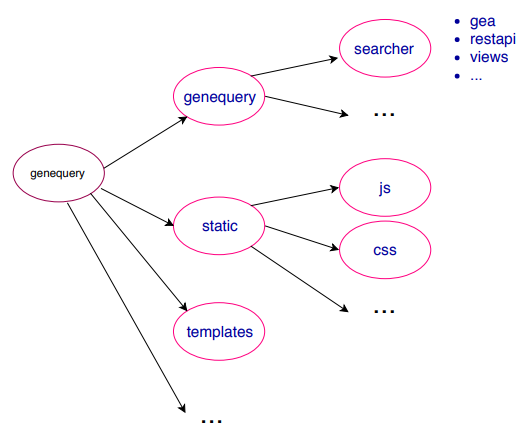
\includegraphics[width=0.8\textwidth]{genequery-web.png}
\end{figure}

Классы из пакета \textit{searcher} были расширены для получения и обработки названий модулей генов. В пакеты \textit{js} и \textit{css}, отвечающие за представление данных, также были добавленны изменения ~-- реализовано само представление модулей, выделены жирным шрифтом значимые части названий, отрегулирована ширина итоговой таблицы и т.д. Пару шаблонов было изменено в пакете \textit{templates} ~-- например, название новой версии сервиса.   

\section{Представление результатов пользователю}

Пользователь выбирает организм и вводит соответствующий ему набор генов, как показано на рисунке~\ref{clientRequest}. Система выдает ответ в виде статистически значимых модулей (рисунки~\ref{clientResponseShort} и ~\ref{clientResponseTable}), в которых найдены совпадающие гены. Список отсортирован в порядке возрастания логарифма \textit{adj.p-value ≤ 0.01}. Как можно видеть, информация, которую получает пользователь по каждому модулю, также включает в себя название эксперимента, название модуля, число перекрытий генов (рисунок~\ref{clientResponseOverlap}), ссылку на эксперимент и возможность загрузки таблицы с дифференциальной экспрессией данного модуля.

\begin{figure}[!h]
    \caption{Пример поиска для молекулярного пути ответа на гипоксию.}\label{clientRequest}
    \centering
    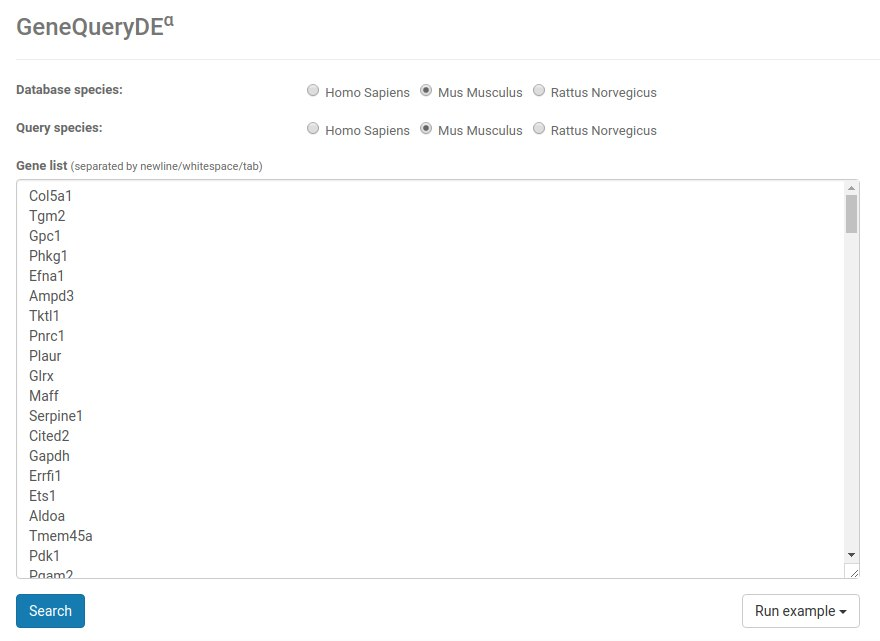
\includegraphics[width=0.9\textwidth]{request.jpg}
\end{figure}

\begin{figure}[!h]
    \caption{Результат поиска ~-- количество найденных модулей генов для молекулярного пути ответа на гипоксию.}\label{clientResponseShort}
    \centering
    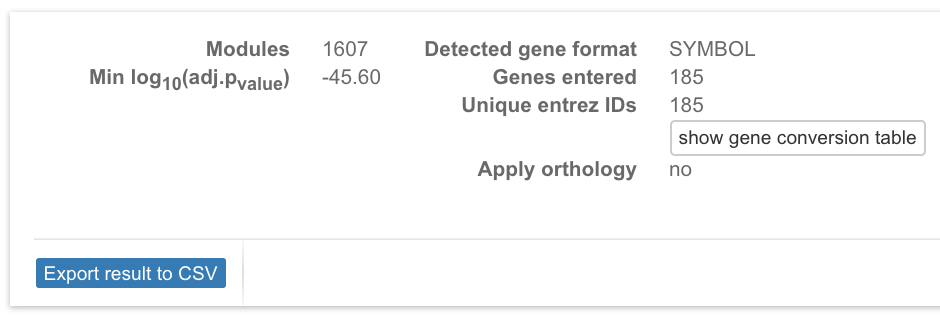
\includegraphics[width=0.7\textwidth]{responseModulesNumber}
\end{figure}

\begin{figure}[!h]
    \caption{Результат поиска ~-- список модулей для молекулярного пути ответа на гипоксию.}\label{clientResponseTable}
    \centering
    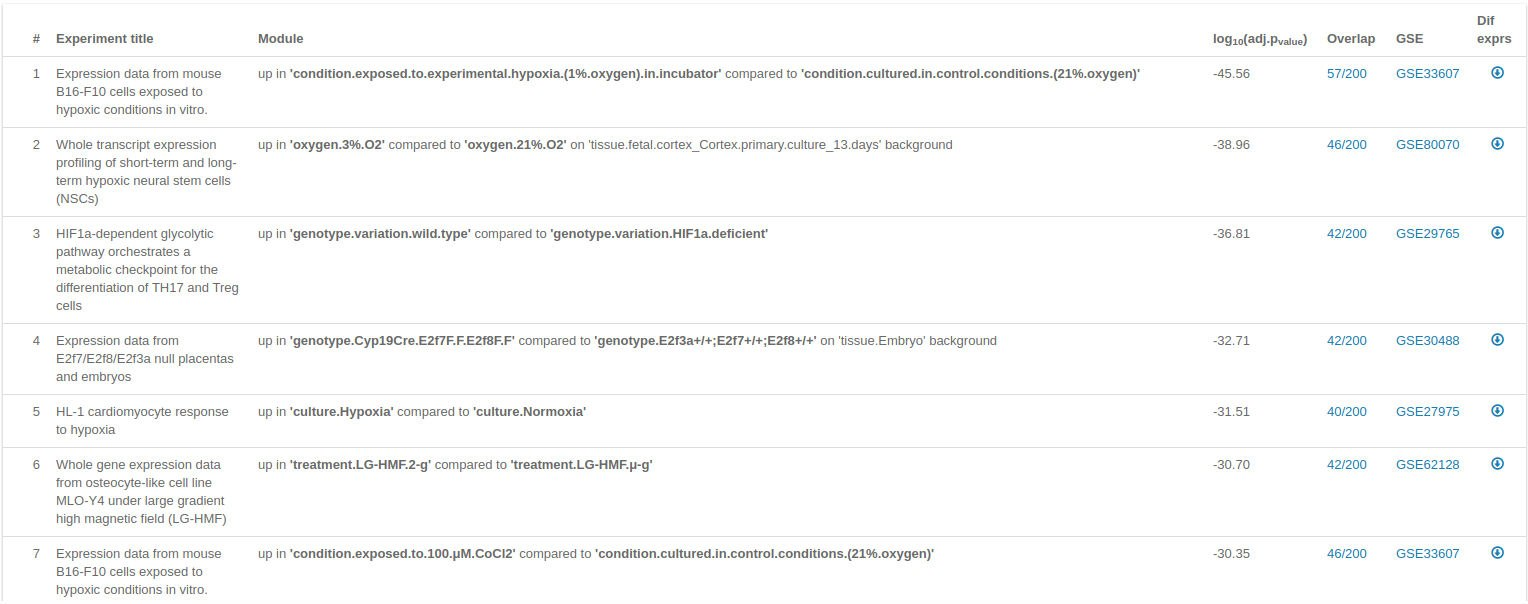
\includegraphics[width=1\textwidth]{responseModulesList.jpg}
\end{figure}

\begin{figure}[!h]
    \caption{Результат поиска ~-- перекрытие генов первого модуля, найденного для молекулярного пути ответа на гипоксию.}\label{clientResponseOverlap}
    \centering
    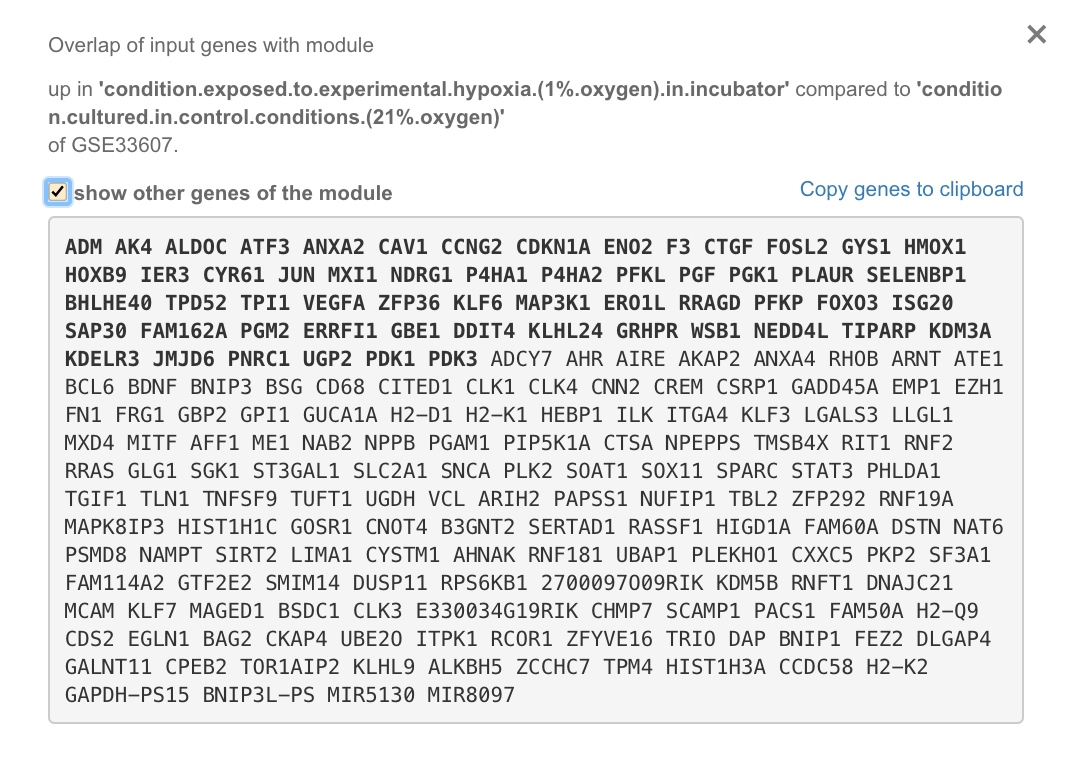
\includegraphics[width=1\textwidth]{overlap}
\end{figure}

Название модуля включает в себя два биологических состояния, на основании которых была вычисленна дифференциальная экспрессия, и условия, которые не менялись.

Например, \textit{up in} \textbf{\lq oxygen.3\%.O2\rq } \textit{compared to} \textbf{\lq oxygen.21\%.O2\rq} \textit{on \lq tissue.fetal.cortex\_Cortex.primary.culture\_13.days\rq~background} ~-- ответ на гипоксию. Здесь гены при \textbf{\lq oxygen.3\%.O2\rq} реагируют против \textbf{\lq oxygen.21\%.O2\rq} на основании условий, присутствующих в обоих экспериментах. 

Как можно видень на рисунке~\ref{clientResponseTable} первый найденный модуль называется \textit{up in \lq condition.exposed.to.experimental.hypoxia(1\%.oxygen).in.incubator\rq compared to ​\lq condition.cultured.in.control.conditions.(21\%.oxygen)\rq}. Учитывая, что гипоксия ~-- это недостаток кислорода, логично наблюдать в найденных модулях генов, модули, в названиях которых фигурирует разница в кислороде. Последующие модули тоже так или иначе включают эту информацию. 

\section{Контейнеризация}

В соответствии с документацией docker \cite{DockerDock} был создан Dockerfile для построения образа и впоследующем контейнера с сервисом. Используя данную технологию, проект GeneQueryDE, состоящий из front-end и back-end частей был упакован в docker-контейнер с доступом к данным с сервера ~-- к модулям генов, \textit{.gmt} файлам и аннотациям к ним. Контейнер запущен, т.ч. сервис доступен по адресу \textit{http://genome.ifmo.ru/genequery-de}.  

\chapterconclusion

В данной главе были описаны структура и интерфейс сервиса GeneQueryDE, способ выдачи результата и пример запроса-ответа. Сказано о различиях, внесенных в версию GeneQueryDE по сравнению с GeneQuery. Также обозначена возможность доступа к сервису посредством интернета. 

\chapter{СРАВНЕНИЕ И АНАЛИЗ РЕЗУЛЬТАТА}

\section{Сравнение GeneQuery с GeneQueryDE по числу данных}

На рисунке~\ref{GSEnumbers} представленно сравнение сервисов по количеству пар GSE+GPL, для которых в последствии были построены модули генов. Как можно увидеть, помимо совпадающих экспериментов, проанализированных в обоих сервисах, также много уникальных GSE, обработанных только в одном из проектов. Причем в GeneQueryDE обработано больше. Если для вида Rattus Norvegicus количество уникальных GSE примерно равно в обоих проектах, то, например, для Mus Musculus, сервис GeneQueryDE предоставляет в 2.8 раза больше экспериментов, доступных для поиска, чем версия GeneQuery. 

\begin{figure}[!h]
    \caption{Сравнение по парам GSE+GPL.}\label{GSEnumbers}
    \centering
    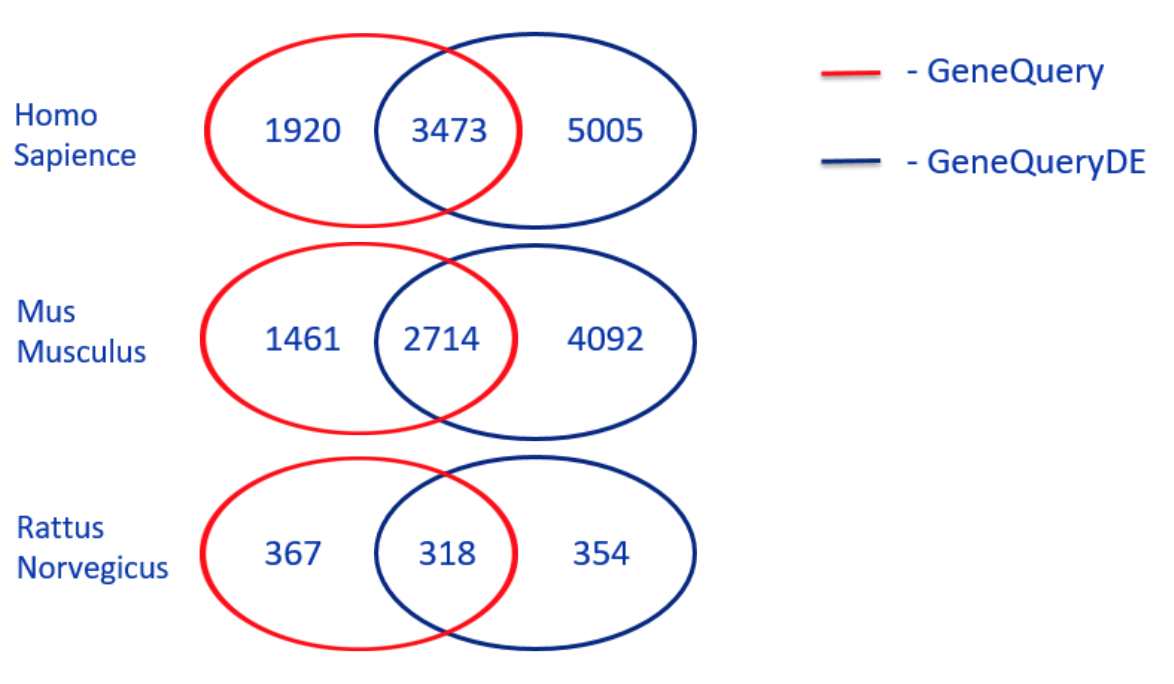
\includegraphics[width=0.8\textwidth]{GSEnumbers}
\end{figure}

В таблице~\ref{ModulesTable} представлены различия в итоговом числе модулей, полученных для двух сервисов. Видно, что сервис GeneQueryDE работает с гораздо большим количеством данных, чем альтернативная версия.

\begin{table}[!h]
    \caption{Сравнение по модулям генов}\label{ModulesTable}
    \centering
    \begin{tabu}{ |X[l]|*{2}{X[c]|}}
        \cline{2-3}
        \multicolumn{1}{c|}{} & \multicolumn{2}{c|}{Модули экспрессии генов}\\ \cline{2-3}
        \multicolumn{1}{c|}{} & GeneQuery & GeneQueryDE\strut\\ \hline
        Homo Sapience & 117497 & 620216 \\ \hline
        Mus Musculus & 82371 & 201240 \\ \hline 
        Rattus Norvegicus & 13560 & 22868 \\ \hline
    \end{tabu}
\end{table}

\section{Сравнение сервисов}

В данном разделе приведено сравнение существующих проектов с GeneQueryDE. А именно, сервисов GeneQuery, GEOracle, ARCHS4 и GEO Profiles. Как видно из таблицы~\ref{ServicesTable} все сервисы выполняют разные функции, принимая на вход различные аргументы. Сервис GeneQueryDE делает свою уникальную работу ~-- ищет модули дифференциальной экспрессии генов, перекрывающиеся с запросом пользователя, и выдает их, ранжируя в порядке статистической значимости.

\begin{sidewaystable*}
    \caption{Сравнение сервисов}\label{ServicesTable}
    \centering
    %\begin{tabu}{ |X[l]|*{3}{X[c]|}}
    \begin{tabu}{ |X[l]|m{6.7cm}|m{6.7cm}|m{6.7cm}|}
    \cline{2-4}
        \multicolumn{1}{c|}{} & \cellcolor{Gray} Входные данные & \cellcolor{Gray} Обрабатываемые виды & \cellcolor{Gray} Результаты работы \strut\\ 
        \hline
        \cellcolor{Gray} GeneQuery & Набор генов & \begin{itemize}
            \item Homo Sapience
            \item Mus Musculus
            \item Rattus Norvegicus
        \end{itemize} & \begin{itemize}
            \item Перекрытия генов
            \item Тепловые карты экспрессии генов
        \end{itemize}\\ 
        \hline
        \cellcolor{darkgray} GeneQueryDE & \cellcolor{darkgray} Набор генов & \cellcolor{darkgray} \begin{itemize}
            \item Homo Sapience
            \item Mus Musculus
            \item Rattus Norvegicus
        \end{itemize} & \cellcolor{darkgray} \begin{itemize}
            \item Перекрытия генов
            \item Модули дифференциальной экспрессии
        \end{itemize}\\ 
        \hline 
        \cellcolor{Gray} GEOracle & Набор экспериментов & Без ограничений & \begin{itemize}
            \item Числовые значения дифференциальной экспрессии
            \item Тепловые карты зависимости экспериментов от генов
        \end{itemize}\\ 
        \hline
        \cellcolor{Gray} ARCHS4 & \begin{itemize}
            \item Ген
            \item Набор генов в верхней/нижней регуляции
            \item (доп.параметры: ткани, органы)
        \end{itemize} & \begin{itemize}
            \item Homo Sapience
            \item Mus Musculus
        \end{itemize} & \begin{itemize}
            \item Информация о гене
            \item Средняя экспрессия гена
        \end{itemize}\\ 
        \hline
        \cellcolor{Gray} GEO Profiles & \begin{itemize}
            \item Ген
            \item Эксперимент
            \item Организм
            \item Свободный текст
        \end{itemize} & Без ограничений & \begin{itemize}
            \item Эксперименты с аннотациями
            \item Информация о генах
        \end{itemize}\\ 
        \hline
    \end{tabu}
\end{sidewaystable*}

\chapterconclusion

В данной главе были подведены итоги созданного сервиса GeneQueryDE, а именно произведено его сравнение с альтернативной версией по количеству обрабатываемых данных и сравнение с существующими проектами. 
  

%% Заключение
\startconclusionpage

В результате данной работы:
\begin{itemize}
    \item Построены модули дифференциальной экспрессии генов для видов Homo Sapience, Mus Musculus, Rattus Norvegicus.
    \item Сервис GeneQuery расширен до версии GeneQueryDE, обеспечивающей интерфейс доступа к модулям генов. 
    \item Число экспериментов, доступных для поиска, увеличено по сравнению с GeneQuery. 
    \item Разработанное решение было упаковано в контейнер.
    \item Сервис GeneQueryDE был развернут по адресу: \textit{http://genome.ifmo.ru/genequery-de}.​
\end{itemize}

\printmainbibliography

\end{document}
